\chapter{Implementation and testing}
\label{cha:implandtest}

A MMS robot equipped with a depth acquisition system is a particularly well suited tool to perform tasks with a high degree of autonomy. The high volume of environmental information provided by a depth sensor allows the robot to successfully operate in an unstructured and changing environment without human guidance. In this work, the task which the robot has to solve fully autonomously is the problem of finding a predefined object in its working environment. This problem required implementing two mechanisms for depth data processing. The first was the detection of obstacles, in order to ensure save movement of the mobile platform and the second one was the recognition of the object to accomplish the final task. The Point Cloud Library (PCL) \cite{Rusu_ICRA2011_PCL, pcl} was used to implement the depth data analysis on the robot. PCL is an open source project for 3D point cloud processing. The library contains a vast array of state-of-the-art algorithms for filtering, feature estimation, segmentation, registration and model fitting. Apart from the PCL, the OpenMP \cite{openmp} library for multithreading functionality and the FLANN \cite{flann} library for approximate nearest neighbours algorithm are utilised in the project. A detailed description of the developed autonomous control mode is provided in the following sections.

%---------------------------------------------------------------------------

\section{Hardware setting}
\label{sec:setting}

The first issue encountered during the development of the autonomous mode was adequate positioning of the depth camera. As mentioned in section \ref{sec:3dsum}, the selected RGB-D sensor, Asus Xtion Pro operating range starts from $0.8m$. In practice, however, the first proper measurements are returned from a distance of $0.5m$, which is still a relatively high value compared to the dimensions of the whole robot. For this reason, the camera position and field of view determines the size of objects that can be used as targets. Moreover, the RGB-D camera location is also crucial during obstacle detection. The system should be able to determine whether it is possible to displace an entire width of the platform forward. While moving ahead, the analysed area is desired to be large enough that the robot could react to obstacle on time and avoid collision. The region close to the front of the platform should also be examined, as obstacles are likely to occur there during platform rotation.

The mounting point of the RGB-D camera has been selected in place of an end-effector of the larger manipulator. This setting has allowed for reproducible and convenient adjustments of the camera pose. The Figure \ref{fig:fov} presents a simplified view of camera setting relative to the mobile platform. The manipulator is positioned in the plane compliant with the drawing and only the joints relevant to this plane are specified. The joint angles $\theta_1, \theta_2, \theta_3$ were experimentally selected to meet the previously established field of view requirements. In such setting, the robot is able to perceive the full dimensions of small sized objects, such as a coffe mug, which is sufficient for further processing purposes.

\usetikzlibrary{patterns}
\usetikzlibrary{calc}
\usetikzlibrary{decorations.pathmorphing}
%Small:
%L0 = 250?,L1 = 143, L2 = 98 + 58 = 156, L3 = 50 + 35
%Big:
%L0 = 250?,L1 = 240, L2 = 127 + 58 = 185, L3 = 50 + 35 = 85
% Define the kinematic parameters of the three link manipulator.
\def\scale{0.01}
\def\MinDepth{\scale*550}
\def\Lzero{\scale*250}
\def\thetaone{120}
\def\Lone{\scale*250}
\def\thetatwo{-60}
\def\Ltwo{\scale*185}
\def\thetathree{-30}
\def\Lthree{\scale*85}
\pgfmathsetmacro\SensorTheta{\thetaone + \thetatwo + \thetathree}
\pgfmathsetmacro\SensorHeight{\Lzero + \Lone * sin(180 - \thetaone) + \Ltwo * sin(\thetaone + \thetatwo) + \Lthree * sin(\thetaone + \thetatwo + \thetathree)}

\newcommand{\nvar}[2]{%
    \newlength{#1}
    \setlength{#1}{#2}
}

% Define a few constants for drawing
\nvar{\dg}{0.3cm}
\def\dw{0.25}\def\dh{2.5}%{1.3}
\nvar{\ddx}{1.5cm}

% Define commands for links, joints and such
\def\link{\draw [double distance=1.5mm, thick] (0,0)--}
\def\joint{%
    \filldraw [fill=white] (0,0) circle (5pt);
    \fill[black] circle (2pt);
}
\def\grip{%
	
    \filldraw [fill=white, thick] (0cm,\dg) rectangle (3mm,-\dg);    
    
    %\draw[ultra thick](0cm,\dg)--(0cm,-\dg)--(3mm,-\dg)--(3mm,\dg) -- cycle;
    \fill (1.5mm, -\dg) -- +(-1.5mm,-1.5mm) -- +(1.5mm,-1.5mm);
    %\fill (0cm, -0.5\dg)+(0cm,1.5pt) -- +(0.6\dg,0cm) -- +(0pt,-1.5pt);
}
\def\robotbase{%
    \draw[thick, yscale = 1.923](-0.5,0) rectangle (0.5,-0.3);
    \draw[thick, yscale = 1.923](-1,-0.3) -- (0.6+0.15,-0.3)  -- (0.6+0.15+0.4,-0.65) -- (0.6+0.15,-1) -- (-1,-1);
	\draw[decorate, decoration={snake, segment length=0.43cm,amplitude=.9}, yscale = 1.923] (-1,-0.3)  -- (-1,-1); 
    \filldraw [fill=white, thick] (0.35 - 0.22,-0.9*1.923) circle (0.4*1.923);    
    
}


\newcommand{\ground}[1]{
    \fill[white] (-1.5,-\dh) rectangle (#1,-\dh-0.5);
    \draw (-1.5,-\dh)-- (#1,-\dh);
    \fill[pattern=north east lines] (-1.5,-\dh) rectangle (#1,-\dh-0.5);
}

% Draw an angle annotation
% Input:
%   #1 Offset (optional)
%   #2 Angle
%   #3 Label
% Example:
%   \angann{30}{$\theta_1$}
\newcommand{\angann}[3][\ddx]{%
    \begin{scope}[red]
    \draw [dashed, red] (0,0) -- (1.2*#1,0pt);
    \draw [->, shorten >=3.5pt] (#1,0pt) arc (0:#2:#1);
    % Unfortunately automatic node placement on an arc is not supported yet.
    % We therefore have to compute an appropriate coordinate ourselves.
    \node at (#2/2-2:#1+8pt) {#3};
    \end{scope}
}

% Draw line annotation
% Input:
%   #1 Line offset (optional)
%   #2 Line angle
%   #3 Line length
%   #5 Line label
% Example:
%   \lineann[1]{30}{2}{$L_1$}
\newcommand{\lineann}[4][0.5]{%
    \begin{scope}[rotate=#2, blue,inner sep=2pt]
        \draw[dashed, blue!40] (0,0) -- +(0,#1)
            node [coordinate, near end] (a) {};
        \draw[dashed, blue!40] (#3,0) -- +(0,#1)
            node [coordinate, near end] (b) {};
        \draw[|<->|] (a) -- node[fill=white] {#4} (b);
    \end{scope}
}

% Draw view
% Input:
%   #1 Line offset (optional)
%   #2 Line angle
%   #3 Line length
%   #5 Line label
% Example:
%   \lineann[1]{30}{2}{$L_1$}
\newcommand{\view}[4]{%
    \begin{scope}[rotate=#2, blue,inner sep=2pt]
        \draw[dashed, blue!40] (0,0) -- +(0,#1)
            node [coordinate, near end] (a) {};
        \draw[dashed, blue!40] (#3,0) -- +(0,#1)
            node [coordinate, near end] (b) {};
        \draw[|<->|] (a) -- node[fill=white] {#4} (b);
    \end{scope}
}

\begin{figure}[H]

\begin{centering}

\begin{tikzpicture}
    \lineann[-1.75]{-90}{\dh}{$L_0$}
    \robotbase
    \angann[1cm]{\thetaone}{$\theta_1$}
    \lineann[0.7]{\thetaone}{\Lone}{$L_1$}
    \link(\thetaone:\Lone);
    \joint
    \begin{scope}[shift=(\thetaone:\Lone), rotate=\thetaone]
        \angann{\thetatwo}{$\theta_2$}
        \lineann[-0.5]{\thetatwo}{\Ltwo}{$L_2$}
        \link(\thetatwo:\Ltwo);
        \joint
        \begin{scope}[shift=(\thetatwo:\Ltwo), rotate=\thetatwo]
            \angann{\thetathree}{$\theta_3$}
            \lineann[0.7]{\thetathree}{\Lthree}{$L_3$}
            \draw [dashed, red,rotate=\thetathree] (0,0) -- (1.2\ddx,0pt);
            \link(\thetathree:\Lthree);
            \joint
            \begin{scope}[shift=(\thetathree:\Lthree), rotate=\thetathree]
                \grip
                \begin{scope}[shift={(1.5mm,-\dg)}, rotate=-90]
                

				\begin{scope}[rotate=-\SensorTheta, blue,inner sep=2pt]
     			    \draw[dashed, blue!40] (0,0) -- +(0,8.75)
     			        node [coordinate] (a) {};
    				    \draw[dashed, blue!40] (\SensorHeight,0) -- +(0,8.75)
    				        node [coordinate] (b) {};
			        \draw[|<->|] (a) -- node[fill=white] {$H$} (b);
 			    \end{scope}                      
                
				\pgfmathsetmacro\by{\SensorHeight/cos(\SensorTheta)}
				\pgfmathsetmacro\ha{\SensorHeight/cos(\SensorTheta-22.5)}
				\pgfmathsetmacro\hc{\SensorHeight/cos(\SensorTheta+22.5)}
				\pgfmathsetmacro\ay{\ha * cos(-22.5)}
				\pgfmathsetmacro\ax{\ha * sin(-22.5)}
				\pgfmathsetmacro\cy{\hc * cos(22.5)}
				\pgfmathsetmacro\cx{\hc * sin(22.5)}
                \draw[dashed] (0,0) -- (\by,0);
                \coordinate(c) at (\cy,\cx);
                \coordinate(a) at (\ay,\ax);

                \draw (0,0) -- (c);
                \draw (0,0) -- (a);
                
                \node[above right = -0.2](b) at (\MinDepth,\MinDepth*0.4142) {$C$};
                \node[left =-0.1](b) at (\MinDepth,-\MinDepth*0.4142) {$D$};
                \node[right=0.95](cn) at (\cy -1,\cx -1) {$B$};
                \node[right=0.87](an) at (\ay -1,\ax -1) {$A$};
                \fill[pattern=dots] (\MinDepth,-\MinDepth*0.4142) -- (a) -- (c) -- (\MinDepth,\MinDepth*0.4142) -- cycle;

	            \end{scope}
            \end{scope}
        \end{scope}
    \end{scope}
    \ground{10}
\end{tikzpicture}

\end{centering}
\caption{Field of view}
\label{fig:fov}
\end{figure}

%---------------------------------------------------------------------------

\section{Obstacle detection implementation}
\label{sec:objavoid}

Knowledge of the camera field of view facilitates the first stage of depth data processing, the obstacle detection. According to it, the view acquired from the sensor can be further adjusted to detect objects only in the designated area. The full, implemented processing pipeline, including this view adjustments, is presented in the Figure \ref{fig:detectpipe}.

\begin{figure}[H]
\begin{center}
\begin{tikzpicture}
  [node distance = 5mm,auto,every node/.style={rectangle,draw,align=center, font=\footnotesize}]
  
  \node (down) at (1,10) {Downsampling};
  \node[right=of down] (plane) {Plane model \\ Extraction};
  \node[right=of plane] (trans) {Affine \\ Transformation};
  \node[right=of trans] (pass) {Passthrough \\ Filtering};
  \node[right=of pass] (outlier) {Outlier \\ Removal};

  \foreach \from/\to in {down/plane, plane/trans, trans/pass, pass/outlier}
    \draw[->] (\from) -- (\to);

\end{tikzpicture}

\caption{Implemented obstacle detection pipeline}

\label{fig:detectpipe}

\end{center}
\end{figure}

Depth sensors provide a high volume of information, which has to be analysed online with a limited computing resources. Therefore, the first processing step was to reduce the amount of data by downsampling. For this purpose, a voxel grid filter with a leaf size of $1cm \times 1cm \times 1cm$ has been applied. Due to the reduced number of points, this step has significantly accelerated further processing stages, thus allowing to generate sufficiently fast response on obstacle emergence.


By design, the robot is intended to work in the indoor environment. A significant feature of such environment is the planar surface of the floor. Therefore, by fitting a plane model to the acquired point cloud, it is possible to determine the  area belonging to the ground, and thus free of obstacles. The RANSAC algorithm implementation, available in the PCL library, was used to estimate the plane model parameters $A,B,C,D$, given by Equation \ref{eq:planemodel}. 
The maximum iterations of the algorithm are set to $1000$, and distance threshold between the point and the model is set to $1cm$. After the fitting, all of the model inliers are removed from the point cloud. This step thus leaves only the points that potentially belong to an obstacle. On the other hand, if the RANSAC algorithm fails to fit the model, it is assumed that the entire view is occluded by obstacles and the procedure returns positive detection.  The Figure \ref{fig:floorcut} illustrates an example of plane model extraction.

\begin{figure}
\centering
\begin{subfigure}{.3\textwidth}
  \centering
  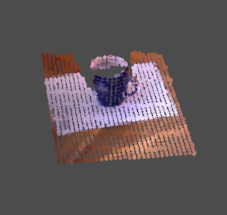
\includegraphics[width=.8\linewidth]{fig/floorcut1}
  \caption{Input point cloud}
  \label{fig:sub1}
\end{subfigure}%
\begin{subfigure}{.3\textwidth}
  \centering
  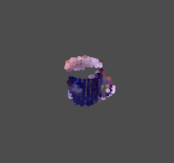
\includegraphics[width=.8\linewidth]{fig/floorcut2}
  \caption{Plane extraction result}
  \label{fig:sub2}
\end{subfigure}
\caption{An example of floor extraction for a mug}
\label{fig:floorcut}
\end{figure}

The next processing step, the volume of interest (VoI) extraction, involves separation of a cuboidal space from the remaining point cloud. The dimensions of the extracted cuboid directly correspond to the total height and width of the robot, and the maximum distance at which the system is supposed to react to obstacles. As shown in Figure \ref{fig:fov}, the camera is pointing to the floor at a certain angle. This direction is represented by a Z-axis of the coordinate system in the acquired point cloud. To enable the VoI extraction with the specified dimensions, the coordinate system of the cloud is rotated by an angle $\theta$ around the X-axis, such that the Z-axis of the resultant coordinate frame is parallel to the floor. This transformation can be based on the angle $\theta_1 - \theta_2 - \theta_3$, from Section \ref{sec:setting}. However, because of the vibrations caused by the platform movement, a more accurate solution is to use the previously calculated plane model. A vector $\vec{n}$ normal to a plane \ref{eq:planemodel} is given by:
\begin{equation}
 \vec{n} = \frac{1}{\sqrt{A^2+B^2+C^2}} \cdot \left[
\begin{array}{c}
A\\
B\\
C\\
\end{array}
\right] 
\end{equation}
The third coordinate $n_z$ of the normal vector $\vec{n}$ satisfies $n_z = sin(\theta)$ and the final rotation matrix is given by:

\begin{equation}
R_x=\left[\begin{array}{ccc}
      1 & 0 & 0  \\
      0 & \sqrt{1 - n_z^2} & -n_z  \\
      0 & n_z & \sqrt{1 - n_z^2}  \\
    \end{array}\right]
\end{equation}
After viewpoint transformation, the VoI is extracted by applying a Passthrough filter along X and Z axes of the received cloud. The filtration ranges have been experimentally selected to $[-0.3m, 0.3m]$ along the X axis, which corresponds to the robot width, and $[0m, 0.55m]$ along the Z axis, which represent the maximal obstacle distance.

The last stage of the obstacle detection processing is the outlier removal. The RadiusOutlierRemoval class from PCL is utilised for this purpose. The search radius of this filter is selected to $r = 10cm$, and the number of $r$-neigbours, below which the query point is considered as an outlier, is set to $10$. Such setting allows to reduce the number of noise in the point cloud and the final result of obstacle detection is then based on the remaining number of points. If the processed point cloud contains more than $50$ points, a positive obstacle detection is returned. This threshold allows to successfully detect small objects, such as a box of matches, while discarding all of the remaining measurement errors.

	

%---------------------------------------------------------------------------

\section{Object recognition implementation}
\label{sec:detection}

In addition to ensuring safe movement of the robot, the previously described obstacle  detection pipeline also performs most of the necessary preprocessing steps for object recognition. Upon obstacle detection, the resulting point cloud contains points that belong only to the objects in the scene, thus further processing is directly applied to that cloud. 

Two different approaches of object recognition were implemented during the project. The first one uses an analytical model of the objects shape and allows to recognize objects with simple geometric structures, such as spheres or cylinders. The second, more general method is based on the objects detailed model, acquired during 3D scanning. Despite the differences, both of these approaches share some common preprocessing steps, including the normal estimation and cluster segmentation. To determine the normal vectors for a given cloud, the NormalEstimationOMP class, available in PCL library, is used. This class exploits the OpenMP library to parallelize computations, which significantly accelerates the process of normal estimation. 

	It is assumed that during the exploration of the environment, the robot can encounter a scene with multiple objects. In such situation, it is convenient to isolate individual items and analyse them separately. For this purpose, a greedy algorithm of Euclidean Cluster Extraction is applied to the point cloud. The cluster tolerance is set to $5cm$. This parameter, due to the nature of the euclidean segmentation, imposes a minimal distance of $5cm$ between object surfaces. As a result of the segmentation process, a vector of point clouds is obtained and further analysis is applied to each of its elements.
	
	In case of the first, geometric primitives based approach, the model fitting is performed directly on the point clouds obtained after the segmentation. The SACSegmentationFromNormals class from PCL library is used during the fitting process. In this approach, the recognition of two geometric shapes is implemented, the sphere and the cylinder. As a result of fitting a sphere, the algorithm returns four optimized parameters: three coordinates of the sphere center point and its radius.
	
For the cylinder model, seven parameters are obtained, including the radius, three coordinates of its axis direction and three coordinates of a point lying on that axis. Furthermore, in order to distinguish cylindrical objects with different heights, a few additional steps are required after the model is found. Firstly, the point cloud coordinate system is transformed so as to cover the cylinder axis with the Z-axis. Next, two points with minimum and maximum $z$-coordinates are found with the getMinMax3D function from PCL. Finally, the resulting height $h$ of the cylinder is given by the difference of those coordinates, that is $h = z_{max} - z_{min}$. Figure \ref{fig:cylinder} illustrates an example of fitting a cylinder model (highlighted with red) to a point cloud.

\begin{figure}[H]
\centering
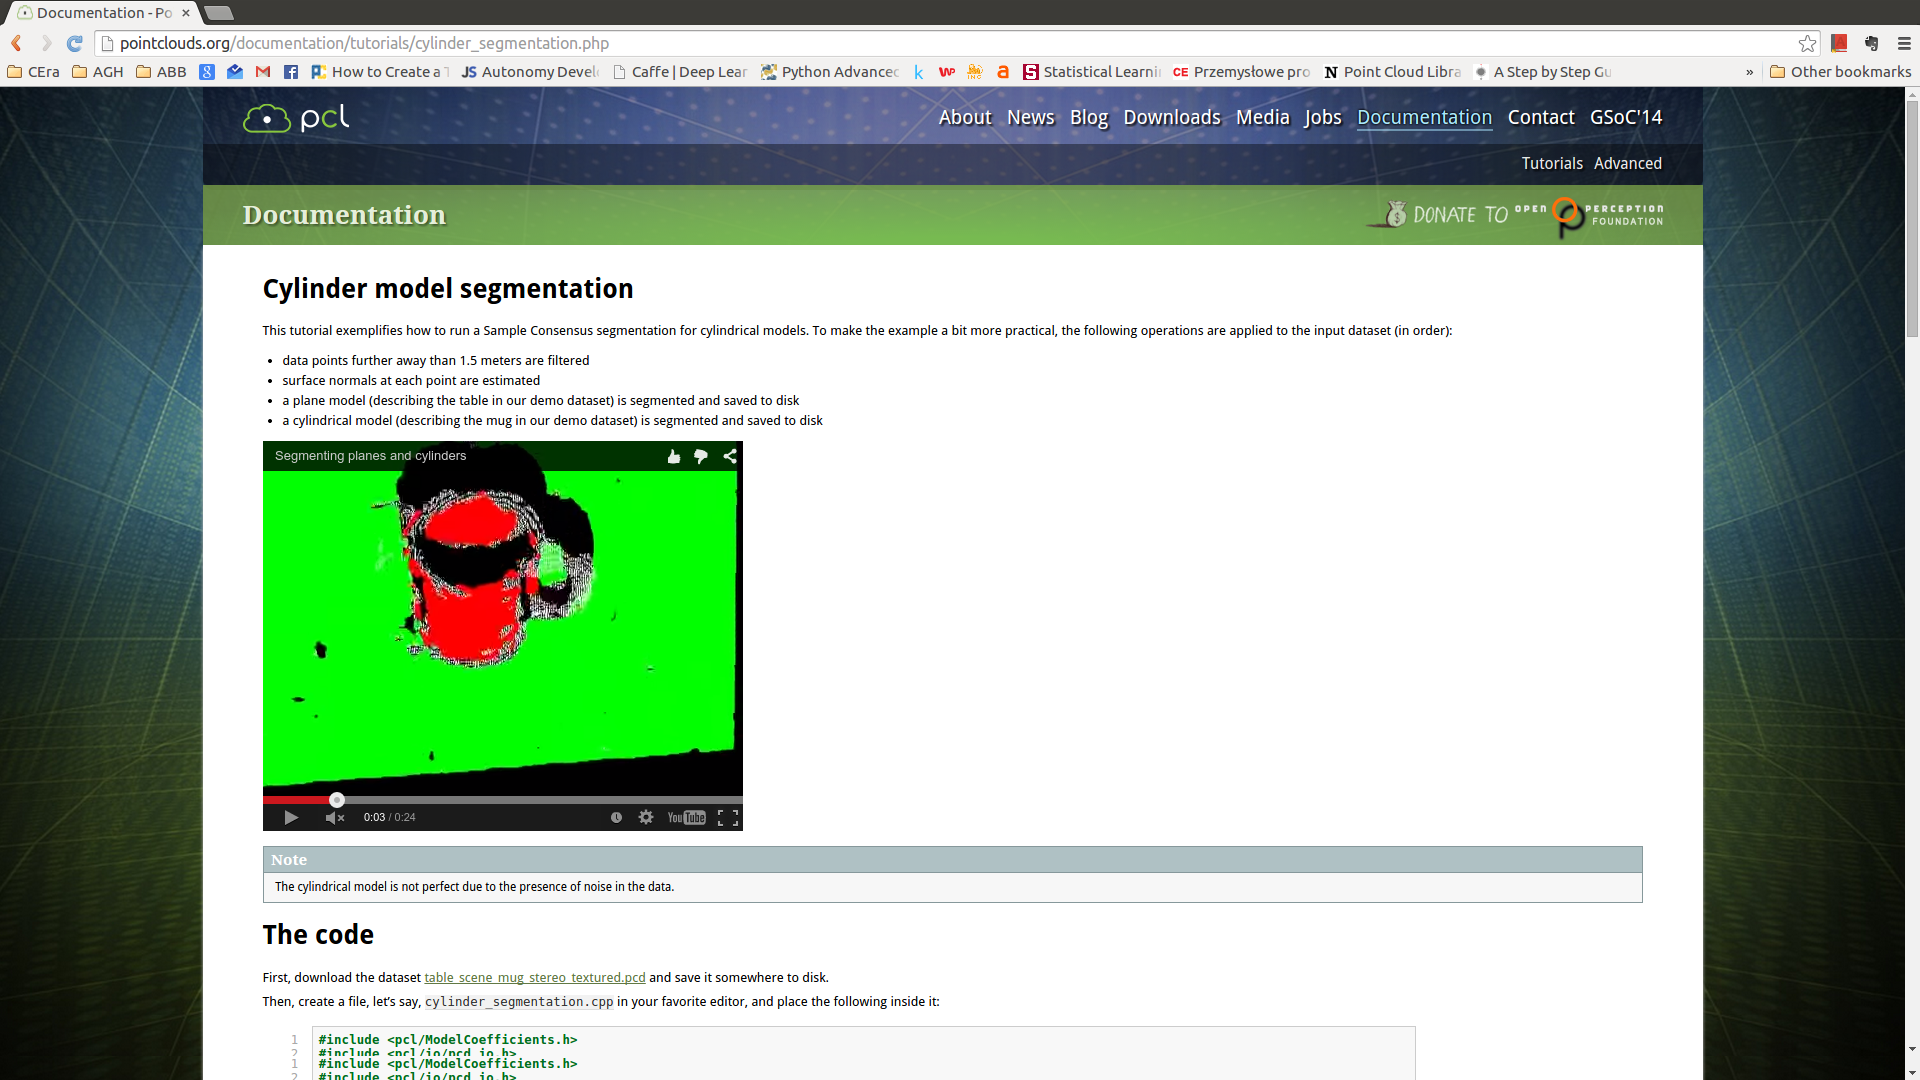
\includegraphics[width=0.3\textwidth]{fig/cylinder}
\caption{Cylinder model fitting example \cite{pcl}}
\label{fig:cylinder}
\end{figure}

The second, general method of object recognition utilises the global recognition pipeline described in Section \ref{sec:pipeline}. This selection is justified by the fact, that the global approach requires a set of partial object scans as a training set, which can be easily acquired with available hardware. The VFH descriptor, estimated by the PCL VFHEstimation class, is used to compare the point clusters. To obtain the training data set, a series of scans by the RGB-D camera are taken from different, characteristic views of the object. For each of these scans, the VFH descriptor is calculated and added to a KD-Tree structure, which is then saved to the hard drive. During the recognition process, for a given VFH descriptor of a cluster, a nearest-neighbour search is performed in the KD-Tree structure, by the \textit{knnSearch} method from the FLANN library. If the resultant $L_1$ distance between the neighbour and the segment VFH is less than a given threshold, the procedure returns positive object recognition. The further post-processing steps, listed in Section \ref{sec:pipeline}, which estimate the 6DOF pose of an object were omitted, as the task of the robot is to only determine the existence of a given object.

%---------------------------------------------------------------------------

\section{The autonomous control mode}
\label{sec:autonomy}

Procedures of obstacle detection and object recognition provide the necessary tools to achieve the stated task of autonomous finding of predefined objects. The autonomous mode was implemented in the form of a C++ application, executed on the NVIDIA Jetson TK1 platform. This application communicates with the control server via HTTP requests, as described in Section \ref{sec:soft}. For this purpose, the HTTP POST and GET methods from cpp-netlib \cite{netlib} library are utilised. All of the required communication request are encapsulated in the form of a Robot class object. The methods of this class enable the realization of such actions as driving forward, platform rotation, stopping and setting the manipulator joints in given positions. 

The depth data processing procedures described in preceding sections posses a significant amount of configurable parameters. To avoid having to recompile the code with every parameter customization, all of the relevant constants are included in a configuration file in a XML format. The path to this XML file is specified as a command-line argument of the application, together with the name of  the target to search for. The configuration file contains also information on the recognition method type and the path to the training set for the specified target name.

\begin{figure}[H]
\begin{centering}

\begin{tikzpicture}[->,>=stealth',shorten >=1pt,auto,node distance=3cm,
  thick,main node/.style={circle,draw,font=\sffamily\Large\bfseries}]

  \node[main node] (1) {S};
  \node[main node] (2) [above left of=1] {M};
  \node[main node] (3) [above right of=1] {T};

  \path[every node/.style={font=\sffamily\small}]
    (1) edge [bend left] node {$D\wedge\overline{R}$} (2)
        edge node[left] {$\overline{D}$} (3)
    (2) edge node [right] {$R$} (1)
        edge [bend left] node[above] {$\overline{D}$} (3)
    (3) edge node [above] {$D\wedge\overline{R}$} (2)
        edge [bend left] node {$R$} (1);
\end{tikzpicture}

\caption{State diagram of the autonomous mode}
\label{fig:statetrans}

\end{centering}
\end{figure}

The system operation outline is presented in the Figure \ref{fig:statetrans}, in the form of a state diagram. Three different states of motion are distinguished: forward movement (\textbf{F}), turning (\textbf{T}) and stopping (\textbf{S}). 
At the time of entrance to each of the \textbf{F}, \textbf{T}, \textbf{S} states, a corresponding command is sent to the control server. Transitions between these states are determined by the logical values returned from the procedures of obstacle detection (\textit{D}) and object recognition (\textit{R}). The robot moves forward if there are no obstacles in front of it, stops if it encounters the target object and turns if it discovers an obstacle. The direction of turning is selected in a pseudo-random manner at each newly encountered obstacle. In this way, the system is able to explore the whole working environment. 

%---------------------------------------------------------------------------

\section{Testing environment and results}
\label{sec:testing}


The implemented obstacle avoidance system was tested in a household environment, among objects of everyday usage. The robot was able to move flawlessly between obstacles, such as furniture, boxes or even people. On the other hand, some minor drawbacks of the system were noticed. Firstly, the assumption of the flat surface of the floor is not always true for such environment. Low doorsteps, for example, were treated as obstacles and limited the exploration area to only one room. Another important limitation is the fact, that the utilised depth sensor does not provide proper measurements for highly reflective or transparent surfaces. Therefore, obstacles with such properties pose a potential threat to the system operation.

\begin{figure}[H]
\centering
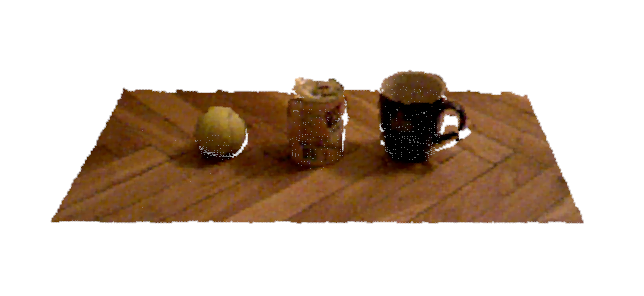
\includegraphics[width=0.5\textwidth]{fig/targetswhite}
\caption{A point cloud with all of the target objects}
\label{fig:targets}
\end{figure}

Three search targets were selected to test the implementation of the object recognition methods. A tennis ball and a tin can for sphere and cylinder model fitting approach and a coffee mug for general object recognition. The selected targets are presented in the Figure \ref{fig:targets}. To generate the training set for global descriptor matching, eight scans of the coffee mug were taken with manual object rotation by an angle increment of \SI{45}{\degree}. Those snapshots were then processed to extract the object points and calculate the VFH descriptors. One of such partial object scans, with its VFH histogram is shown in the Figure \ref{fig:mugvfh}.

\begin{figure} [H]
\centering
\begin{subfigure}{.2\textwidth}
  \centering
  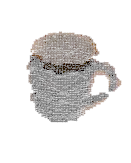
\includegraphics[width=.8\linewidth]{fig/mugvfh}
  \caption{Partial target scan}
  \label{fig:mugvfh1}
\end{subfigure}%
\begin{subfigure}{.7\textwidth}
  \centering
  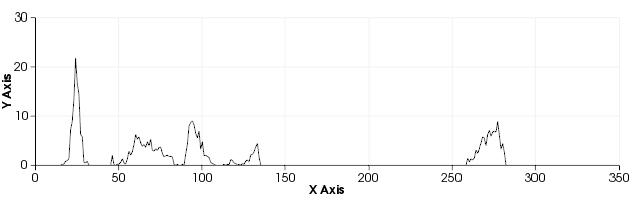
\includegraphics[width=.8\linewidth]{fig/mug3vfh}
  \caption{VFH histogram}
  \label{fig:mugvfh2}
\end{subfigure}
\caption{A partial scan of the target and its VFH descriptor}
\label{fig:mugvfh}
\end{figure}

Each of the implemented methods provided different recognition performance. The best results of the established task were obtained with the spherical model of the tennis ball, which was recognized in most of the cases. This is justified by the fact, that this model possess the smallest number of optimized parameters. The most difficult aspect of testing the object recognition implementation, which requires further improvement, was to properly set all of the thresholding parameters for the depth data processing procedures. 

The RANSAC shape model fitting is governed by the distance threshold between the accepted inliers and the model. This parameter is used to specify the expected inaccuracy of the acquired point cloud.  In case of the tennis ball target, the model is successfully matched with tolerance of $5mm$. The cylindrical model, on the other hand, required much higher tolerance of about $3cm$ to return positive model recognition. Unfortunately, such high tolerance resulted i.e. in cylinders fitted to furniture edges. A possible improvement of this method performance requires further tuning of parameters, such as the normal estimation radius. In case of the recognition method based on the VFH descriptor, the results were also unsatisfactory and further research has to be conducted to improve its performance. Most probably, this was caused by the fact, that the training set was generated from insufficient descriptive angles. In future, a pan-tilt device is planned to be utilised for object scanning from a large number of distinct rotations.